\documentclass[tikz, border=2mm]{standalone}
\usepackage{tikz}
\usepackage{polyomino}

\definecolor{color1}{rgb}{0.36, 0.54, 0.66}
\definecolor{color2}{rgb}{0.54, 0.81, 0.94}
\definecolor{color3}{rgb}{0.13, 0.67, 0.8}
\definecolor{color4}{rgb}{0.0, 0.5, 0.69}
\definecolor{color5}{rgb}{0.4, 0.6, 0.8}
\definecolor{color6}{rgb}{0.0, 0.58, 0.71}

\pgfkeys{
  /polyomino,
  p={F}{style={color1, draw=black, line width=0.5pt, fill opacity=0.6, dotted}},
  p={I}{style={color2, draw=black, line width=0.5pt, fill opacity=0.6, dotted}},
  p={L}{style={color3, draw=black, line width=0.5pt, fill opacity=0.6, dotted}},
  p={N}{style={color4, draw=black, line width=0.5pt, fill opacity=0.6, dotted}},
  p={O}{style={color5, draw=black, line width=0.5pt, fill opacity=0.6, dotted}},
  p={T}{style={color6, draw=black, line width=0.5pt, fill opacity=0.6, dotted}}
}

\begin{document}
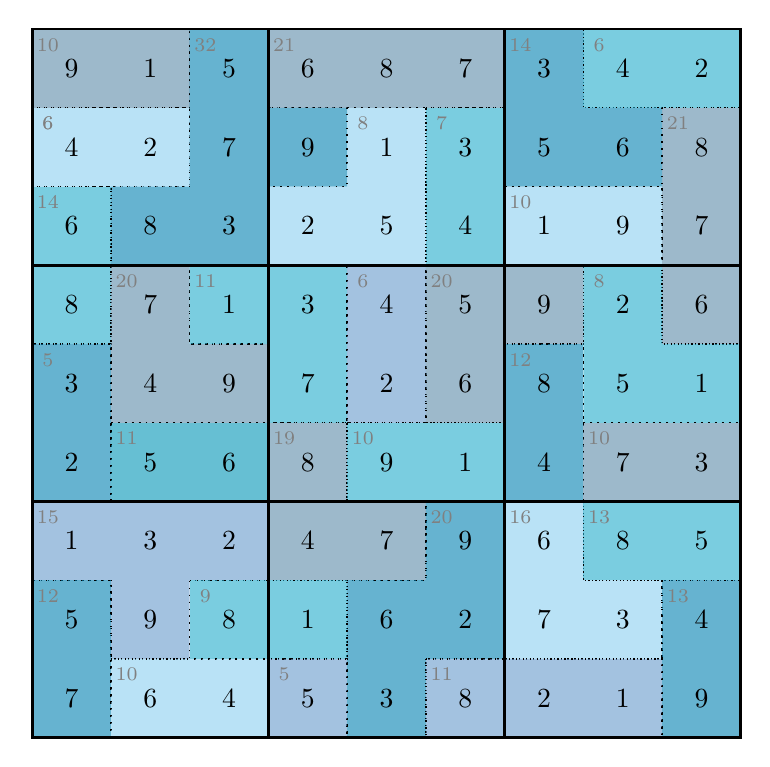
\begin{tikzpicture}
\polyomino[
  %grid
]{
  FFNFFFNLL,
  IINNILNNF,
  LNNIILIIF,
  LFLLOFFLF,
  NFFLOFNLL,
  NTTFLLNFF,
  OOOFFNILL,
  NOLLNNIIN,
  NIIONOOON
}

\draw[color=gray] (0.2,8.8) node {{\scriptsize{$10$}}};
\draw[color=gray] (0.2,7.8) node {{\scriptsize{$6$}}};
\draw[color=gray] (0.2,7.8) node {{\scriptsize{$6$}}};
\draw[color=gray] (0.2,6.8) node {{\scriptsize{$14$}}};
\draw[color=gray] (0.2,4.8) node {{\scriptsize{$5$}}};
\draw[color=gray] (0.2,2.8) node {{\scriptsize{$15$}}};
\draw[color=gray] (0.2,1.8) node {{\scriptsize{$12$}}};
\draw[color=gray] (1.2,5.8) node {{\scriptsize{$20$}}};
\draw[color=gray] (1.2,3.8) node {{\scriptsize{$11$}}};
\draw[color=gray] (1.2,0.8) node {{\scriptsize{$10$}}};
\draw[color=gray] (2.2,8.8) node {{\scriptsize{$32$}}};
\draw[color=gray] (2.2,5.8) node {{\scriptsize{$11$}}};
\draw[color=gray] (2.2,1.8) node {{\scriptsize{$9$}}};
\draw[color=gray] (3.2,8.8) node {{\scriptsize{$21$}}};
\draw[color=gray] (3.2,3.8) node {{\scriptsize{$19$}}};
\draw[color=gray] (3.2,0.8) node {{\scriptsize{$5$}}};
\draw[color=gray] (4.2,7.8) node {{\scriptsize{$8$}}};
\draw[color=gray] (4.2,5.8) node {{\scriptsize{$6$}}};
\draw[color=gray] (4.2,3.8) node {{\scriptsize{$10$}}};
\draw[color=gray] (5.2,7.8) node {{\scriptsize{$7$}}};
\draw[color=gray] (5.2,5.8) node {{\scriptsize{$20$}}};
\draw[color=gray] (5.2,2.8) node {{\scriptsize{$20$}}};
\draw[color=gray] (5.2,0.8) node {{\scriptsize{$11$}}};
\draw[color=gray] (6.2,8.8) node {{\scriptsize{$14$}}};
\draw[color=gray] (6.2,6.8) node {{\scriptsize{$10$}}};
\draw[color=gray] (6.2,4.8) node {{\scriptsize{$12$}}};
\draw[color=gray] (6.2,2.8) node {{\scriptsize{$16$}}};
\draw[color=gray] (7.2,8.8) node {{\scriptsize{$6$}}};
\draw[color=gray] (7.2,5.8) node {{\scriptsize{$8$}}};
\draw[color=gray] (7.2,3.8) node {{\scriptsize{$10$}}};
\draw[color=gray] (7.2,2.8) node {{\scriptsize{$13$}}};
\draw[color=gray] (8.2,7.8) node {{\scriptsize{$21$}}};
\draw[color=gray] (8.2,1.8) node {{\scriptsize{$13$}}};

% Thick Borders 
\draw [line width=1pt,color=black] (0,0) -- (9,0) -- (9,9) -- (0,9) -- cycle;
\draw [line width=1pt,color=black] (3,0) -- (3,9);
\draw [line width=1pt,color=black] (6,0) -- (6,9);
\draw [line width=1pt,color=black] (0,3) -- (9,3);
\draw [line width=1pt,color=black] (0,6) -- (9,6);

% Solution
\draw[color=black] (0.5,0.5) node {$7$};
\draw[color=black] (1.5,0.5) node {$6$};
\draw[color=black] (2.5,0.5) node {$4$};
\draw[color=black] (3.5,0.5) node {$5$};
\draw[color=black] (4.5,0.5) node {$3$};
\draw[color=black] (5.5,0.5) node {$8$};
\draw[color=black] (6.5,0.5) node {$2$};
\draw[color=black] (7.5,0.5) node {$1$};
\draw[color=black] (8.5,0.5) node {$9$};

\draw[color=black] (0.5,1.5) node {$5$};
\draw[color=black] (1.5,1.5) node {$9$};
\draw[color=black] (2.5,1.5) node {$8$};
\draw[color=black] (3.5,1.5) node {$1$};
\draw[color=black] (4.5,1.5) node {$6$};
\draw[color=black] (5.5,1.5) node {$2$};
\draw[color=black] (6.5,1.5) node {$7$};
\draw[color=black] (7.5,1.5) node {$3$};
\draw[color=black] (8.5,1.5) node {$4$};

\draw[color=black] (0.5,2.5) node {$1$};
\draw[color=black] (1.5,2.5) node {$3$};
\draw[color=black] (2.5,2.5) node {$2$};
\draw[color=black] (3.5,2.5) node {$4$};
\draw[color=black] (4.5,2.5) node {$7$};
\draw[color=black] (5.5,2.5) node {$9$};
\draw[color=black] (6.5,2.5) node {$6$};
\draw[color=black] (7.5,2.5) node {$8$};
\draw[color=black] (8.5,2.5) node {$5$};

\draw[color=black] (0.5,3.5) node {$2$};
\draw[color=black] (1.5,3.5) node {$5$};
\draw[color=black] (2.5,3.5) node {$6$};
\draw[color=black] (3.5,3.5) node {$8$};
\draw[color=black] (4.5,3.5) node {$9$};
\draw[color=black] (5.5,3.5) node {$1$};
\draw[color=black] (6.5,3.5) node {$4$};
\draw[color=black] (7.5,3.5) node {$7$};
\draw[color=black] (8.5,3.5) node {$3$};

\draw[color=black] (0.5,4.5) node {$3$};
\draw[color=black] (1.5,4.5) node {$4$};
\draw[color=black] (2.5,4.5) node {$9$};
\draw[color=black] (3.5,4.5) node {$7$};
\draw[color=black] (4.5,4.5) node {$2$};
\draw[color=black] (5.5,4.5) node {$6$};
\draw[color=black] (6.5,4.5) node {$8$};
\draw[color=black] (7.5,4.5) node {$5$};
\draw[color=black] (8.5,4.5) node {$1$};

\draw[color=black] (0.5,5.5) node {$8$};
\draw[color=black] (1.5,5.5) node {$7$};
\draw[color=black] (2.5,5.5) node {$1$};
\draw[color=black] (3.5,5.5) node {$3$};
\draw[color=black] (4.5,5.5) node {$4$};
\draw[color=black] (5.5,5.5) node {$5$};
\draw[color=black] (6.5,5.5) node {$9$};
\draw[color=black] (7.5,5.5) node {$2$};
\draw[color=black] (8.5,5.5) node {$6$};

\draw[color=black] (0.5,6.5) node {$6$};
\draw[color=black] (1.5,6.5) node {$8$};
\draw[color=black] (2.5,6.5) node {$3$};
\draw[color=black] (3.5,6.5) node {$2$};
\draw[color=black] (4.5,6.5) node {$5$};
\draw[color=black] (5.5,6.5) node {$4$};
\draw[color=black] (6.5,6.5) node {$1$};
\draw[color=black] (7.5,6.5) node {$9$};
\draw[color=black] (8.5,6.5) node {$7$};

\draw[color=black] (0.5,7.5) node {$4$};
\draw[color=black] (1.5,7.5) node {$2$};
\draw[color=black] (2.5,7.5) node {$7$};
\draw[color=black] (3.5,7.5) node {$9$};
\draw[color=black] (4.5,7.5) node {$1$};
\draw[color=black] (5.5,7.5) node {$3$};
\draw[color=black] (6.5,7.5) node {$5$};
\draw[color=black] (7.5,7.5) node {$6$};
\draw[color=black] (8.5,7.5) node {$8$};

\draw[color=black] (0.5,8.5) node {$9$};
\draw[color=black] (1.5,8.5) node {$1$};
\draw[color=black] (2.5,8.5) node {$5$};
\draw[color=black] (3.5,8.5) node {$6$};
\draw[color=black] (4.5,8.5) node {$8$};
\draw[color=black] (5.5,8.5) node {$7$};
\draw[color=black] (6.5,8.5) node {$3$};
\draw[color=black] (7.5,8.5) node {$4$};
\draw[color=black] (8.5,8.5) node {$2$};
\end{tikzpicture}
\end{document}
